\chapter{Bundling proteins' dynamics and effects on actin binding proteins}\label{ch:abp-bundle}

\section[Abstract]{Abstract\footnotemark}

This chapter includes work from three papers that are a collaboration with Cristian Suarez, John Winkelman, Jenna Christensen, and Katie Homa in the Kovar lab to understand the role that different bundlers play when it comes to regulating other actin binding proteins. One interest in the Kovar lab is how different proteins sort to the correct F-actin network at the correct time in the cell cycle. All F-actin networks contain at least one crosslinking protein that can link two actin filaments together. These bundling proteins have different kinetics and facilitate different architectures of F-actin. Since bundling proteins can bind along the side of actin filaments and play an important role for a network's architecture, we hypothesized that they would be good candidates for upstream regulators of other actin binding proteins in each network. Furthermore, these bundling proteins can compete or cooperate with each other as well as other actin binding proteins to contribute to the network's architecture. 

In the first paper, in collaboration with Cristian Suarez, we were interested in how long, straight filaments of the filopodia can emerge from the dense, branched lamellipodia. We hypothesized that the bundling protein fascin found in filopodia could inhibit Arp2/3 complex branching. In a collaboration with Jon Winkelman, we were interested in studying the competition between fascin and $\alpha$-actinin that we found is intrinsically determined due to the size of the two bundling proteins. Cristian Suarez and I performed electron microscopy to visualize at a higher resolution the transition state between fascin and $\alpha$-actinin domains. For the third paper, in collaboration with Jenna Christensen and Katie Homa, we were interested in the mechanism of how \textit{S. Pombe} tropomyosin can facilitate $\alpha$-actinin to form more stable bundles. I performed TIRFM with sparsely labeled $\alpha$-actinin to measure its dynamics on F-actin in the presence or absence of tropomyosin. Cristian Suarez analyzed this TIRF data to calculate the spot density of $\alpha$-actinin.

Overall these three works contribute to understanding the role that actin binding proteins, and more specifically bundling proteins, can effect the sorting of actin binding proteins to different F-actin networks, potentially driving the distinct properties of each network. I have presented below the data from the collaborations that I had a role collecting and analyzing and focus on the aspects that are relevant to my contribution. 

\footnotetext{Citations for chapter: [1] Cristian Suarez, Jonathan D. Winkelman, Alyssa J. Harker, Patrick M. McCall, Alisha N. Morganthaler, Margaret L. Gardel, David R. Kovar. Reconsitution of lamellipodia to filopodia transition using pure protein. \textit{In preparation.} [2] Jonathan D. Winkelman, Cristian Suarez, Glen M. Hocky, Alyssa J. Harker, Alisha N. Morganthaler, Jenna R. Christensen, Gregory A. Voth, James R. Bartles, and David R. Kovar. Fascin- and $\alpha$-Actinin-Bundled Networks Contain Intrinsic Structural Features that Drive Protein Sorting. \textit{Current Biology}, 26{20}:2697-2706, October 2016. [3] Jenna R. Christensen, Kaitlin E. Homa, Alisha N. Morganthaler, Cristian Suarez, Alyssa J. Harker, Meghan O'Connell, and David R. Kovar. Tropomyosin and $\alpha$-actinin cooperation inhibits fimbrin association with actin filament networks in fission yeast. \textit{In preparation.}}

\section{Introduction}\label{ch03-introduction}

Many bundling proteins bind cooperatively to sides of filaments, 
meaning that once one bundling protein binds, another of the same 
protein is more likely to bind in the next available binding site 
than random chance \citep{winkelman_fascin-_2016}. This positive 
feedback mechanism facilitates bundle formation as many bundlers can
bind along the length of the two filaments. Additionally, the cooperativity allows continuous domains of the bundlers to form. We were interested in how different bundling proteins sort to different networks and can effect other actin binding protein sorting. We looked at how fascin affects Arp2/3 complex branching, fascin and $\alpha$-actinin competition creates separate domains, and tropomyosin's impact on $\alpha$-actinin binding. 

Bundling proteins have a large effect on the different architectures of 
F-actin networks. Depending on their dynamics and size they can dictate 
the orientation and spacing of filaments in an actin network as well as 
the stability of the bundles themselves. For example, filopodia and lamellipodia are spatially similar but have very distinct filament orientations \citep{blanchoin_actin_2014}. Lamellipodia filaments are branched by Arp2/3 complex and kept short by capping protein. Fimbrin localizes to the lamellipodia and crosslinks these filaments into a dense meshwork. In contrast, filopodia contain long, straight F-actin bundled primarily by fascin \citep{vignjevic_role_2006}. One open question is how Arp2/3 complex is inhibited from nucleating branched filaments on the F-actin within filopodia. The importance of each bundling protein for initiating and maintaining the network to which it localizes remains unclear. 

Another difference in network architecture is in stress fibers compared to filopodia. Filaments are narrowly spaced within filopodia \citep{mattila_filopodia:_2008}, while stress 
fibers have wider spacing due to the main bundling proteins fascin and 
$\alpha$-actinin, respectively. Fascin is a small globular bundling protein compared to the extended homodimer $\alpha$-actinin. We were interested if the intrinsic properties of the bundling proteins themselves could lead to different sorting between bundling proteins and therefore could lead to different architectures within cells. 

Recently we found that two \textit{S. Pombe} bundling proteins, fimbrin and $\alpha$-actinin, can compete only in the presence of an additional side binding protein, tropomyosin. Tropomyosin is a coiled-coil protein that binds along the sides of F-actin and is known to stabilize F-actin as well as effect other actin binding protein binding \citep{perry_vertebrate_2001}. The competition between fimbrin and $\alpha$-actinin in \textit{S. Pombe} is interesting since fission yeast $\alpha$-actinin is an especially poor bundling protein. Additionally in cells, we see that tropomyosin and alpha-actinin localize to the cytokinetic ring where fimbrin mainly localizes to endocytic actin patches. That tropomyosin can bolster $\alpha$-actinin’s bundling properties and competition against fimbrin could be important for the different network architectures and how different actin binding proteins are sorted. 

\section{Results}\label{bundlers-results}

\subsection{Fascin reduces Arp2/3 complex branch density}
Long, straight filaments are found in filopodia which emerge from a dense, branched F-actin network called the lamellipodium. Within the lamelliapodium, actin branches are nucleated by Arp2/3 complex and are kept short by capping protein. We were interested in what factors control the sorting between these two networks that are spatially close together but architecturally distinct. To test our hypothesis that fascin plays a role in reducing Arp2/3 complex branching, we used two-color TIRFM to visualize Arp2/3 branches in the presence and absence of red-labeled fascin (Figure \ref{fig:fascin_branching}A-B). We then measured branch density in the presence and absence of fascin and normalized it to control branch density in the absence of fascin and for the number of filaments in a bundle (Figure \ref{fig:fascin_branching}D). In order to account for small branches that would be nucleated on the sides of fascin-bundled mother filaments and then quickly incorporated into the bundle, we photobleached the actin. This way we could visualize all new growth of actin filaments (Figure \ref{fig:fascin_branching}C). We observe a 2-fold decrease in branch density in the presence of fascin. Therefore, fascin could contribute to the lack of Arp2/3 complex-mediated branch formation on F-actin within filopodia, but it cannot completely block branching alone so other factors must be contributing. 

\begin{figure}
\centering
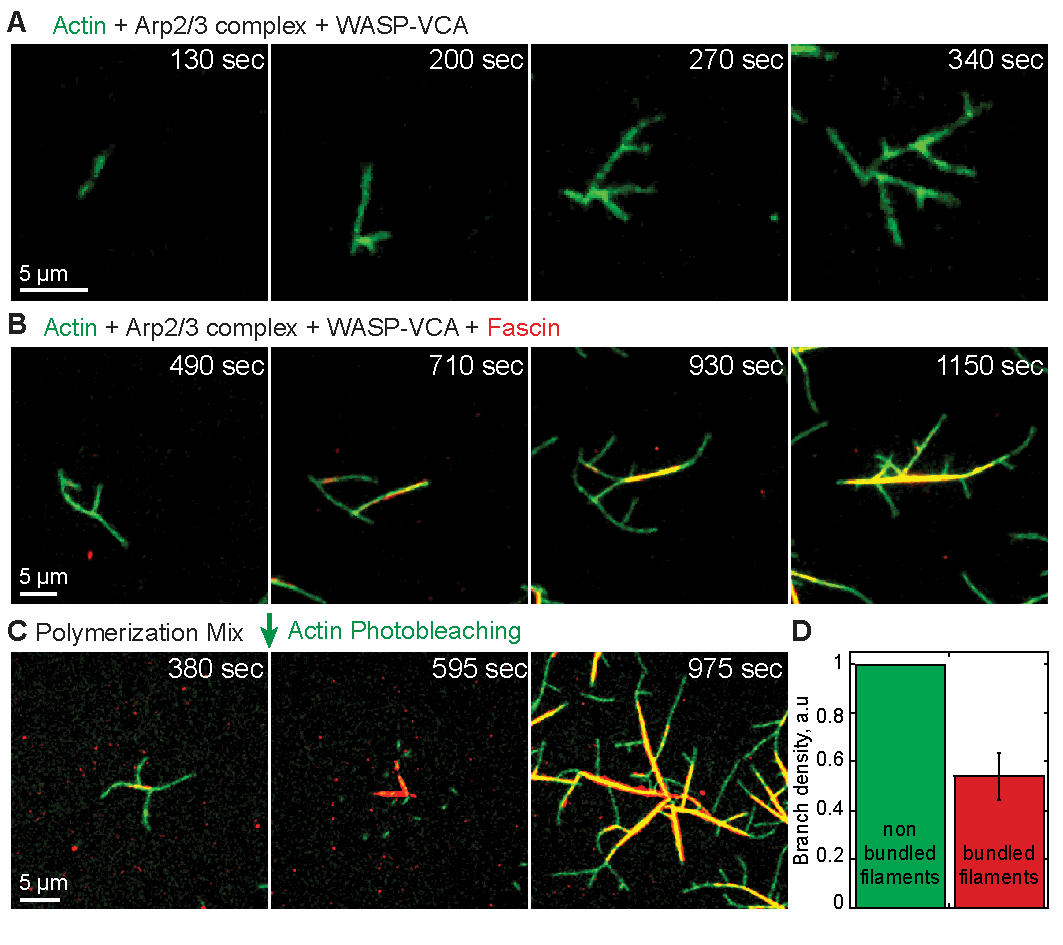
\includegraphics[width=\textwidth]{img/ch03/Thesis_branching.pdf}
\caption[Fascin reduces Arp2/3 complex-mediated branch density]{\textbf{Fascin reduces Arp2/3 complex-mediated branch density} (A-B) Arp2/3 complex-mediated actin polymerization visualized with 1.5 $\mu$M Mg-ATP-actin (15\% Oregon green labeled) polymerized in the presence of 93 nM Arp2/3 complex, 300 nM WASP-VCA as a NPF, and with or without 500 nM TRM-labeled fascin. Arp2/3 complex-mediated actin branches in absence (A) or presence (B) of fascin. Scale bar 5 $\mu$m. (C) 1.5 $\mu$M Mg-ATP-actin (15\% Oregon green labeled) polymerized in the presence of 50 nM Arp2/3 complex, 100 nM WASP-VCA as a NPF, and 500 nM TRM-labeled fascin. To visualize all barbed ends actin fluorescence was photobleached at t = 380 sec. Scale bar 5 $\mu$m. (D) Branch density from single actin filaments and bundled filaments. Error bar, SEM. n = 3. \textbf{Figure modified from Suarez et al. in preparation.}}
\label{fig:fascin_branching}
\end{figure}

\subsection{Fascin and \texorpdfstring{$\alpha$}{alpha}-actinin sort to distinct domains}
Fascin and $\alpha$-actinin have very different structures (Figure \ref{fig:em_fascin_aact}A) and bind to actin using different domains. Fascin is a small globular protein containing  four $\beta$-trefoil domains. In contrast, $\alpha$-actinin forms a long homodimer using two to four spectrin repeats, depending on the homolog, and binds to actin using CH domains. We originally observed fascin and $\alpha$-actinin sorting to distinct domains within actin bundles using \textit{in vitro} TIRFM; however, we were interested in seeing the transition state between the two bundling domains at a higher resolution. Therefore, we performed negative-stain electron microscopy (EM) to visualize preformed actin filaments mixed with either fascin or $\alpha$-actinin alone or both bundling proteins (Figure \ref{fig:em_fascin_aact}B). With fascin alone we see narrow spaced filaments with an interfilament distance of \mytilde8 nm (Figure \ref{fig:em_fascin_aact}D) and a transverse repeat of \mytilde35 nm, which corresponds with one turn of F-actin. $\alpha$-actinin bundles alone have wider spaced filaments (\mytilde32 nm) with a similar transverse repeat of \mytilde35 nm (Figure \ref{fig:em_fascin_aact}C-D). As expected, when both bundlers are mixed together each domain has the characteristics of the respective bundler. The fascin domain is narrow (8 nm) and the $\alpha$-actinin domain is widely spaced (32 nm) (Figure \ref{fig:em_fascin_aact}C-D). We also observe a transition area (142 $\pm$ 53 nm) between the two domains where the filaments become more widely spaced as you transition from a fascin domain to an $\alpha$-actinin domain (Figure \ref{fig:em_fascin_aact}B). 

\begin{figure}
\centering
\includegraphics[width=14cm]{img/ch03/Thesis_EM_fig.png}
\caption[Fascin and \texorpdfstring{$\alpha$}{alpha}-actinin sort to different domains with different interfilament spacing.]{\textbf{Fascin and $\alpha$-actinin sort to different domains with different interfilament spacing.} (A) Structural fold (top) and domain organizations (bottom) showing the four $\beta$-trefoil domains of fascin (PDB 3P53; \citep{jansen_mechanism_2011}) (left) and an $\alpha$-actinin dimer (PDB 1SJJ; \citep{liu_3-d_2004}) (right). ABD, Actin-binding domain; SR, spectrin repeat. (F–H) Electron microscopy (EM) of F-actin bundles negatively stained with uranyl acetate, which were formed from 1.5 $\mu$M actin. (F) Micrographs of bundles with 1 $\mu$M fascin (top), 800 nM $\alpha$-actinin (middle) or both (1 $\mu$M $\alpha$-actinin and 0.25 $\mu$M fascin (bottom). Yellow and green arrowheads indicate fascin and $\alpha$-actinin molecules. L is length of transition zone. Scale bar = 30 nm. (G) Distance of transverse repeat in fascin and $\alpha$-actinin bundles. Error bars indicate SEM; $n\geq10$ bundles. (H) Distance between filaments in a fascin and $\alpha$-actinin bundles. Error bars indicate SEM; $n\geq8$ bundles. \textbf{EM in collaboration with Cristian Suarez. Figure modified from \citep{winkelman_fascin-_2016}}}
\label{fig:em_fascin_aact}
\end{figure}

%check fold values
\subsection{Tropomyosin enhances \texorpdfstring{$\alpha$}{a}-actinin dynamics}
We recently observed that \textit{S. Pombe} tropomyosin, Cdc8, allows $\alpha$-actinin, Ain1, to form more stable bundles. Fimbrin, Fim1, can outcompete either tropomyosin and $\alpha$-actinin to bind to F-actin \citep{christensen_competition_2017}. However, we discovered that together, $\alpha$-actinin and tropomyosin are able to overcome fimbrin. To understand the underlying mechanisms of how this cooperation occurs we studied the single molecule dynamics of $\alpha$-actinin in the presence and absence of tropomyosin using \textit{in vitro} TIRFM. We measured the number of times 0.5\% TMR-labeled $\alpha$-actinin bound F-actin per amount of filament in the presence of polymerizing 1.5 $\mu$M Mg-ATP-actin (10\% Alexa 488-labeled) and with and without 1 $\mu$M unlabeled tropomyosin (Figure \ref{fig:tropo_aact}A-B). We found that $\alpha$-actinin is more dynamic in the presence of tropomyosin. There are 2.3-fold more binding events on F-actin when tropomyosin is also bound (Figure \ref{fig:tropo_aact}C). Therefore, tropomyosin enhances $\alpha$-actinin's association with F-actin and subsequently improves $\alpha$-actinin's bundling properties. 

% get scale bars!!!!!!!!!
\begin{figure}
\centering
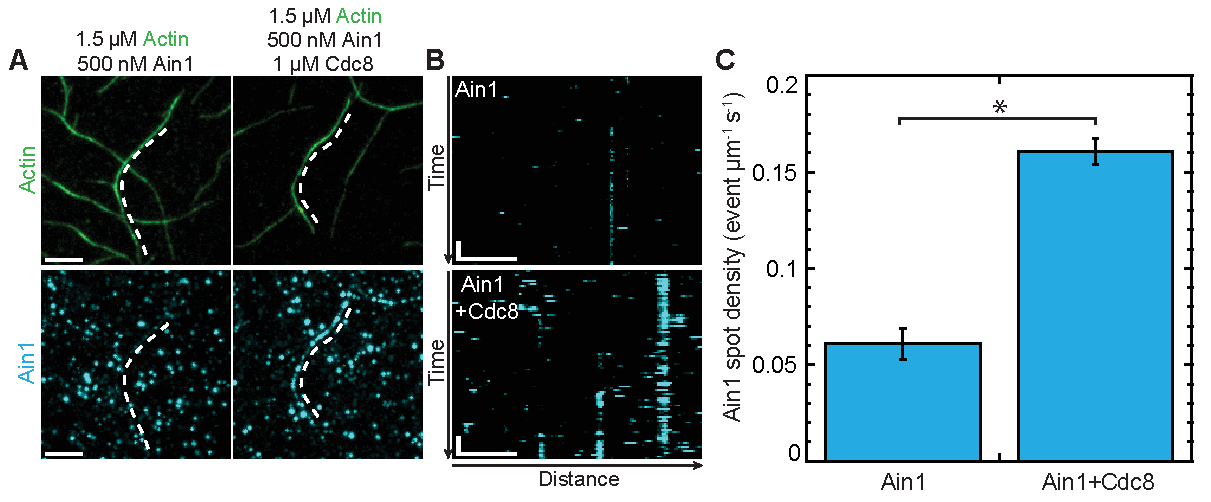
\includegraphics[width=\textwidth]{img/ch03/Thesis_aact_dynamics.pdf}
\caption[Tropomyosin increases \texorpdfstring{$\alpha$}{alpha}-actinin dynamics.]{\textbf{Tropomyosin increases $\alpha$-actinin dynamics.} TIRFM visualization of 1.5 $\mu$M Mg-ATP-actin (10\% Alexa 488-actin) with 500 nM 0.5\% TMR labeled $\alpha$-actinin (Ain1), and 1 $\mu$M unlabeled tropomyosin (Cdc8). (A) Time-lapse micrographs of actin or sparsely labeled $\alpha$-actinin z-projected over 100 frames. Dotted line denotes bundle in both channels. Scale bar, (B) Kymograph of actin bundle length (scale bar, ) over time (time bar, ) showing $\alpha$-actinin spot density. (C) Quantification of $\alpha$-actinin spot density in the presence and absence of tropomyosin. Error bars = SEM. P values (* = 0.04). \textbf{Analysis in collaboration with Cristian Suarez. Figure modified from Christensen et al. in preparation.}}
\label{fig:tropo_aact}
\end{figure}

\section{Materials and Methods}\label{bundlers-matmeth}
\subsection{Visualizing Arp2/3 complex branching in TIRFM}
TIRFM images were collected at 5 s intervals with a cellTIRF 4Line system (Olympus, Center Valley, PA) fitted to an Olympus IX-71 microscope with through-the-objective TIRF illumination and an iXon EMCCD camera (Andor Technology, Belfast, UK). Mg-ATP-actin (15\% Oregon Green-labeled) was mixed with polymerization TIRF buffer [10 mM imidazole (pH 7.0), 50 mM KCl, 1 mM MgCl\textsubscript{2}, 1 mM EGTA, 50 mM DTT, 0.2 mM ATP, 50 $\mu$M CaCl\textsubscript{2}, 15 mM glucose, 20 $\mu$g/mL catalase, 100 $\mu$g/mL glucose oxidase, and 0.5\% (400 centipoise) methylcellulose] to induce F-actin assembly and Arp2/3 complex and NPF WASP-VCA with or without TMR-labeled (red) fascin was added. This mixture was transferred to a flow cell for imaging at room temperature. For two color TIRFM, we cyclically imaged labeled actin (1 frame, 488 nm excitation for 50ms) and TMR-fascin (1 frame, 561 nm excitation for 50ms). The 488 nm laser at high capacity was used to photobleach actin. 

\subsection{Measuring Arp2/3 complex branch density}
First, to calculate the number of filaments in the bundle the fluorescence intensity of actin was recorded for known single filaments 8 frames (40 s) after photobleaching. This was used to calculate the number of filaments in a bundle at this time point by dividing the actin fluorescence by the single filament fluorescence value and was recorded with its corresponding fascin fluorescence value in the 561 channel. The mean gray values for the 561 channel were plotted and a linear equation was fit to calculate the number of filaments in a bundle later in the movie using the TMR-fascin fluorescence. Branch density was calculated from number of observed branches, mean gray value, and length of bundles using TMR-fascin \mytilde 5 minutes after photobleaching. The number of branches formed were counted from the end of photobleaching onwards and this number was divided by the total length of the bundle for branch density. Branches formed before bundling were not counted. The mean gray value was used to calculate the number of filaments in the bundle and this value was used to normalize the branch density to number of filaments.

\subsection{Visualizing F-actin bundles with negative-stain electron microscopy}
Actin (1.5 $\mu$M) was polymerized with either 250–500 nM $\alpha$-actinin, 1–2 $\mu$M fascin, or both bundling proteins for 30 min. This solution was then applied to formvar- and carbon-coated 400 mesh copper grids for 1 min, washed, and negatively stained with 1\% (w/v) uranyl acetate for 1 min, blotted, and dried. Visualization of the bundles using transmission electron microscopy was performed on an FEI Tecnai G2 Spirit microscope at 120 kV. Images were captured on a Gatan 2k $\times$ 2k CCD camera. Bundle parameters were measured using ImageJ.

\subsection{\texorpdfstring{Measuring $\alpha$}{a}-actinin Dynamics in TIRFM}
TIRFM images were collected with a cellTIRF 4Line system (Olympus, Center Valley, PA) fitted to an Olympus IX-71 microscope with through-the-objective TIRF illumination and an iXon EMCCD camera (Andor Technology, Belfast, UK). 1.5 $\mu$M Mg-ATP-actin (10\% Alexa 488 labeled) was mixed with polymerization TIRF buffer [10 mM imidazole (pH 7.0), 50 mM KCl, 1 mM MgCl\textsubscript{2}, 1 mM EGTA, 50 mM DTT, 0.2 mM ATP, 50 $\mu$M CaCl\textsubscript{2}, 15 mM glucose, 20 $\mu$g/mL catalase, 100 $\mu$g/mL glucose oxidase, and 0.5\% (400 centipoise) methylcellulose] to induce F-actin assembly, 0.5 $\mu$M 0.5\% TMR labeled $\alpha$-actinin, and 1 $\mu$M unlabeled tropomyosin. This mixture was transferred to a flow cell for imaging at room temperature. Once the actin had polymerized and formed bundles we imaged once in the 488 channel to visualize the labeled actin (1 frame, 488 nm excitation for 50ms) and then continuously imaged in the 561 channel to visualize the sparsely labeled $\alpha$-actinin (100 frames, 561 nm excitation for 50 ms, \mytilde110 ms interval).
To measure $\alpha$-actinin spot density, we constructed kymographs of bundles for each experiment using ImageJ. $\alpha$-actinin spots were detected in the kymograph as spots at least 4 pixels wide with fluorescence more than 1.25-fold above background fluorescence. We normalized the spot density to the length of actin filaments present in the bundle by measuring each bundle's length, then multiplying the value by the actin fluorescence ratio between the bundle and single filaments. $\alpha$-actinin spot density was determined following the formula: 
\[\rho = \frac{(n/(L\times r))}{t}\]
Where $n$ is the number of $\alpha$-actinin spots detected, $L$ the length of the bundle in $\mu$m, $r$ the actin fluorescence ratio, and $t$ the time of measurement in seconds.


